\documentclass[11pt,twocolumn]{article}
\usepackage{url}
\usepackage{cite}
\usepackage{graphicx}

\begin{document}

\title{Master Thesis Preparation}
\date{\today}
\author{Dominic Bosch \\ Departement Mathematics and Computer Science \\ University of Basel}

\maketitle
\renewcommand{\abstractname}{}
\begin{abstract}
\textbf{Abstract.} This document subsumes the main findings from the preparation work for the masters thesis.
\end{abstract}

\section{Introduction}
The web over time changed its role. In the first stage, it was a passive document storage driven in client-server mode. Using web 2.0 technology in the next phase more and more desk top computer usage went into the web. Today web clouds are proliferating. We anticipate a next change in the near future: The live web or reactive web.
\\
The goal of this project is to enhance the web with rule-based event-condition-action (ECA) mechanisms  such that the web turns itself into an reactive entity. After an analysis of current approaches, a generalized ECA language together with a rule engine should be provided. For test and demonstration purposes, usage scenarios should be specified and new web services should be derived. As a case study, the rule engine should be integrated with the ProBindr software, which is an advanced collaboration platform based on the shelf, binder, and register notion.

\section{Related Work}
In ~\cite{2009-Paschke_Boley-RCER.pdf} the authors supplied general descriptions and classifications of different research efforts in terms of events, rules and reactiveness. Particularly of interest is their identification and summarization of existing research:
 \begin{itemize}
\itemsep-1.5em
  \item Event/Action Logics, Transition Logics and Process Calculi: Events/Actions transit states and effect the lifetime of changeable properties (fluents). Used in \cite{Behrends:2008:EEA:1377798.1377801} to specify complex actions, or in to model the communication behaviour of inbound and outbound message links in rules.
  \item Dynamic/Update/Transition Logics: 
  \item Production Rule Systems:
  \item Active Databases and ECA Rule Systems:
  \item Rule-Based Complex Event Processing and Event Notification Systems: 
\end{itemize}

\subsection{Rule Engines}

\subsubsection{Kinetics Rule Engine}


\subsubsection{Prova}


\subsubsection{OO jDrew}



\subsection{Rule Languages}
\subsubsection{Kinetics Rule Language}


\subsubsection{RuleML}
RuleML~\cite{2006-Boley-RuleML.pdf} is a rule specification standard to express both forward and backward rules for derivation, reaction, rewriting, messaging, verification and transformation. The building blocks of RuleML are predicates, derivation rules, facts, queries, integrity constraints and transformation rules.

The Rule Markup Initiative~\cite{wwwruleml}.


\subsubsection{Reaction RuleML}
Reaction RuleML~\cite{2012-Paschke_etal-ReactionRuleML.pdf} extends RuleML to allow reaction rules and complex event/action messages, e.g. for complex events processing (CEP). It adds various kinds of production, action, reaction and knowledge representation (KR) temporal/event/action logic rules, as well as (complex) event/action messages. It consists of one general reaction rule form that can be specialized, e.g. into production rules, trigger rules, ECA rules or messaging rules. Three different execution styles (active, messaging,  reasoning). Messages define inbound or outbound event messages and are used to interchange events and rule bases. A reaction rule can be globally or locally nested within other reaction or derivation rules.
RuleML Interface Description Language (RuleML IDL) is a sublanguage of Reaction RuleML and allows the description of public rule functions.


\subsubsection{JSON Rules}


\subsection{Frameworks}

\subsubsection{Kynetx}
A framework presented in ~\cite{bookTheLiveWeb}

\subsubsection{Rule Responder}
Rule Responder~\cite{2007-Paschke_etal-RuleResponder.pdf} is a project to extend the Semantic Web towards a Pragmatic Web infrastructure for collaborative human-computer networks, which they call an architecture of a Pragmatic Agent Web (PAW). It supports the formation of virtual groupings and allows semi-automated agents with their individual contexts, decisions and actions. The authors postulate agents empowered with automatic rule-driven data transformation, decision derivation from existing knowledge and reaction according to changed situations or occurred events. The work done in this project concentrates on a layer on top of a rule engine and language, and thus allows for a combination of arbitrary rule-based systems via their framework. This is achieved through the usage of general messge oriented communication interfaces and a platform-independent rule interchange format.
\\
The authors of Rule Responder built their reference system on top of the Mule~\cite{wwwmuleesb} open-source Enterprise Service Bus (ESB) which acts as a communication middleware. The decision to use Mule was made because it goes beyond the typical definition of an ESB by providing a distributable object broker to manage all sorts of service components. Each agent runs its own rbitrary rule engine. For demonstartion purposes Prova and OO jDrew were used to demonstrate the rule interchange between different rule engines.
\\
An investigated use case for Rule Responder was a symposium organization as a virtual organization.

\begin{figure*}[htb]
\begin{center}
%,angle=-90
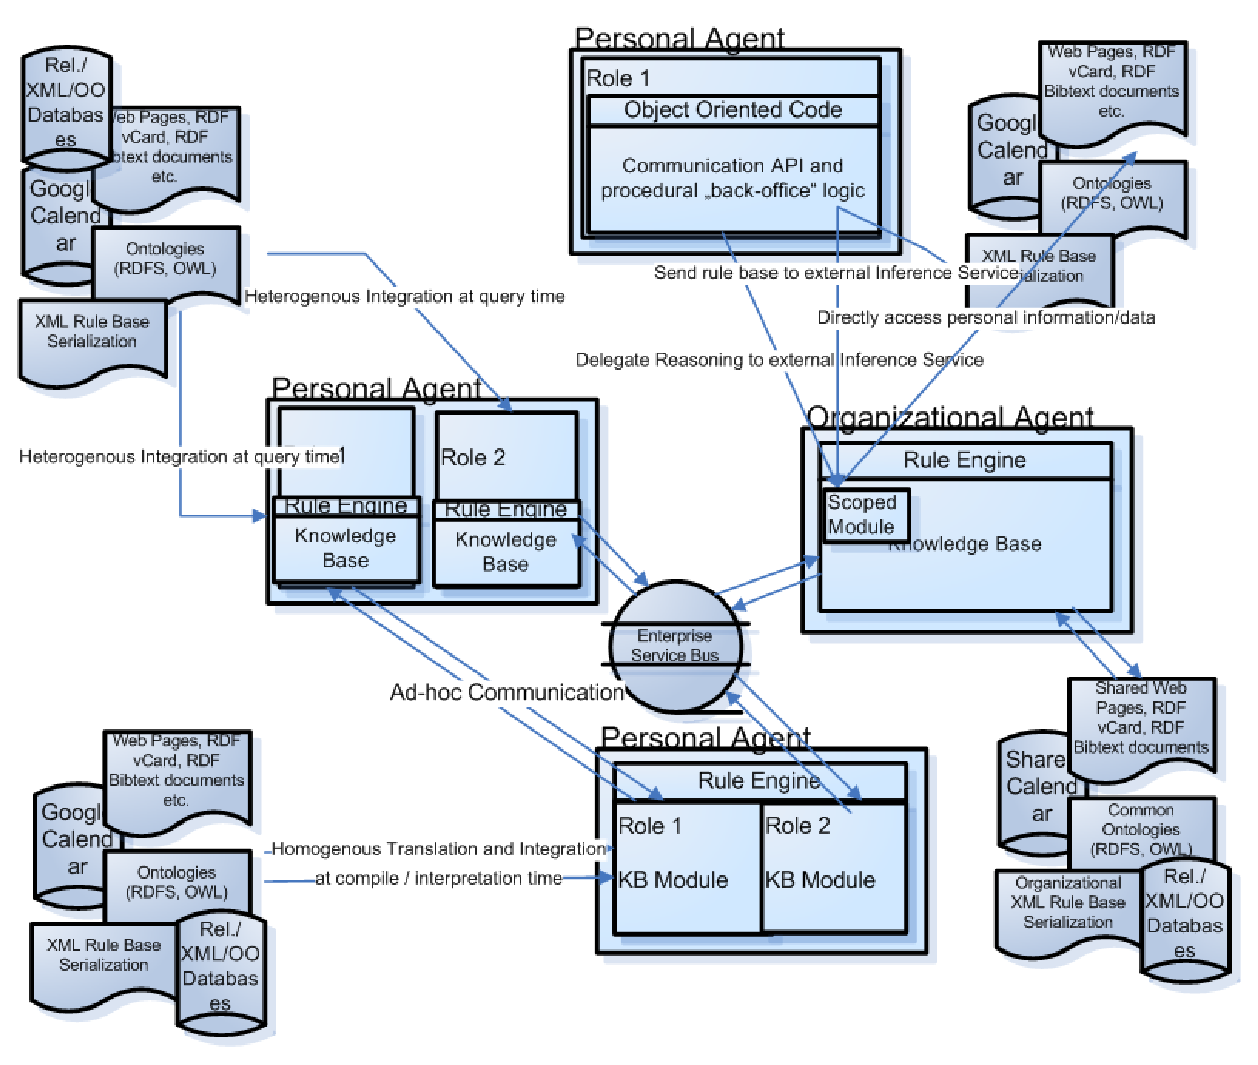
\includegraphics[scale=0.4]{img_rr01}
\caption{Rule Responder Architecture, taken from \cite{2007-Paschke_etal-RuleResponder.pdf}}
\end{center}
\end{figure*}


\subsection{Towards ECA Mashups}
In \cite{2009-Pascalau_Giurca-LWAECARE.pdf}, the founders of JSON Rules~\cite{2008-Giurca_Pascalau-JSON_Rules.pdf} describe a lightweight architecture that allows to react and proact on behalf of events in the ontology of web browsers.



\section{Use Case Study}
In order to verify some of the identified related work, use cases around the succcessor of useKit~\cite{2010-Rizzotti_Burkhart-useKit.pdf}, ProBinder~\cite{wwwprobinder}, have been developed and investigated. 

\section{Conclusion}
There has been a lot of efforts to  


\section{Future Work}


\bibliography{liveweb}
\bibliographystyle{related-work}
\end{document}
